\documentclass[12pt,a4paper]{article}

\usepackage{graphicx}% Include figure files
\usepackage{dcolumn}% Align table columns on decimal point
\usepackage{bm}% bold math
%\usepackage{hyperref}% add hypertext capabilities
%\usepackage[mathlines]{lineno}% Enable numbering of text and display math
%\linenumbers\relax % Commence numbering lines

%\usepackage[showframe,%Uncomment any one of the following lines to test 
%%scale=0.7, marginratio={1:1, 2:3}, ignoreall,% default settings
%%text={7in,10in},centering,
%%margin=1.5in,
%%total={6.5in,8.75in}, top=1.2in, left=0.9in, includefoot,
%%height=10in,a5paper,hmargin={3cm,0.8in},
%]{geometry}

\usepackage{multicol}%Para hacer varias columnas
\usepackage{multicol,caption}
\usepackage{multirow}
\usepackage{cancel}
\usepackage{hyperref}
\hypersetup{
    colorlinks=true,
    linkcolor=blue,
    filecolor=magenta,      
    urlcolor=cyan,
}

\setlength{\topmargin}{-1.0in}
\setlength{\oddsidemargin}{-0.3pc}
\setlength{\evensidemargin}{-0.3pc}
\setlength{\textwidth}{6.75in}
\setlength{\textheight}{9.5in}
\setlength{\parskip}{0.5pc}

\usepackage[utf8]{inputenc}
\usepackage{expl3,xparse,xcoffins,titling,kantlipsum}
\usepackage{graphicx}
\usepackage{xcolor} 
\usepackage{nopageno}
\usepackage{lettrine}
\usepackage{caption}
\renewcommand{\figurename}{Figura}
\usepackage{float}
\renewcommand\refname{Bibliograf\'ia}
\usepackage{amssymb}
\usepackage{amsmath}
\usepackage[rightcaption]{sidecap}
\usepackage[spanish]{babel}

\providecommand{\abs}[1]{\lvert#1\rvert}
\providecommand{\norm}[1]{\lVert#1\rVert}
\newcommand{\dbar}{\mathchar'26\mkern-12mu d}

% CABECERA Y PIE DE PÁGINA %%%%%
\usepackage{fancyhdr}
\pagestyle{fancy}
\fancyhf{}

\begin{document}

\begin{verbatim}
    PROGRAM Pendulo_doble
!*********************************************************************
! Se resuelve el pendulo doble o se intenta ggg
!
!
!**********************************************************************

 REAL*8, DIMENSION(:), ALLOCATABLE :: theta1,omega1,theta2,omega2,t
 REAL*8 :: l1,l2,m1,m2,dt
!

 !print*,"numero de pasos"
 !read*, n   
 n = 500000
 ALLOCATE (theta1(0:n),theta2(0:n),omega1(0:n),omega2(0:n),t(0:n))
!
!
 call inicializa(theta1,theta2, omega1,omega2, t, l1,l2,m1,m2, dt)
 call calcula (theta1, omega1, theta2,omega2,l1,l2,m1,m2, t, n, dt)
 call despliega (theta1,theta2, t, n)
!
END PROGRAM Pendulo_doble
!
!
SUBROUTINE inicializa(theta1,theta2,omega1,omega2, t,l1,l2,m1,m2, dt)
 REAL*8,INTENT (INOUT), DIMENSION(0:n) :: theta1,theta2,omega1,omega2,t
 REAL*8, INTENT (INOUT) :: l1,l2,m1,m2,dt
 !print*,'Angulo inicial del pendulo (en radianes)'
 !read*, theta(0)
 theta1(0) = 0.5d0
 theta2(0) =0.4d0
 !print*,'Velocidad angular inicial del pendulo (en radianes/s)'
 !read*, omega(0)
 omega1(0) = 0.1d0
 omega2(0) =0.1d0
 t(0)=0.d0
 !print*,'Longitud del pendulo (in m)'
 !read*, length
 l1 = 1.d0
 l2 = 1.d0
 m1= 2.d0
 m2 = 2.d0
 !print*, 'Tamaño de paso (en segundos)'
 !read*, dt
 dt=0.001
END SUBROUTINE inicializa
!
!
SUBROUTINE calcula(theta1, omega1, theta2, omega2,l1,l2,m1,m2, t, n, dt)
 INTEGER, INTENT (IN) :: n
 REAL*8, INTENT (IN) ::l1,l2,m1,m2,dt
 REAL*8,INTENT (INOUT), DIMENSION(0:n) :: theta1,omega1, theta2, omega2,t
 REAL*8 :: g,k11,k12,k13,k14,k21,k22,k23,k24
 REAl*8 :: k31,k32,k33,k34,l41,l42,l43,l44,PI
 INTEGER :: i
 PI= 4.*ATAN(1.)
 i= 0
 g= 9.80d0


 DO
 t(i+1) = t(i) + dt
 k11 = dt*omega1(i)
 k21 = dt*omega2(i)
 k31 = dt*OME1(g,m1,m2,theta1(i),theta2(i),omega1(i),omega2(i),l1,l2)
 k41 = dt*OME2(g,m1,m2,theta1(i),theta2(i),omega1(i),omega2(i),l1,l2)
 k12 = dt*(omega1(i)+(0.5d0)*k11)
 k22 = dt*(omega2(i)+(0.5d0)*k21)
 k32 = dt*OME1(g,m1,m2,theta1(i)+(0.5d0)*k11,theta2(i)+(0.5d0)*k21,omega1(i)+(0.5d0)*k31,omega2(i)+(0.5d0)*k41,l1,l2)
 k42 = dt*OME2(g,m1,m2,theta1(i)+(0.5d0)*k11,theta2(i)+(0.5d0)*k21,omega1(i)+(0.5d0)*k31,omega2(i)+(0.5d0)*k41,l1,l2)
 k13 = dt*(omega1(i)+(0.5d0)*k12)
 k23 = dt*(omega2(i)+(0.5d0)*k22)
 k33 = dt*OME1(g,m1,m2,theta1(i)+(0.5d0)*k12,theta2(i)+(0.5d0)*k22,omega1(i)+(0.5d0)*k32,omega2(i)+(0.5d0)*k42,l1,l2)
 k43 = dt*OME2(g,m1,m2,theta1(i)+(0.5d0)*k12,theta2(i)+(0.5d0)*k22,omega1(i)+(0.5d0)*k32,omega2(i)+(0.5d0)*k42,l1,l2)
 k14 = dt*(omega1(i)+(0.5d0)*k13)
 k24 = dt*(omega2(i)+(0.5d0)*k23)
 k34 = dt*OME1(g,m1,m2,theta1(i)+k13,theta2(i)+k23,omega1(i)+k33,omega2(i)+k43,l1,l2)
 k44 = dt*OME2(g,m1,m2,theta1(i)+k13,theta2(i)+k23,omega1(i)+k33,omega2(i)+k43,l1,l2)

 theta1(i+1) = theta1(i)+((1/6.d0)*(k11+((0.5d0)*(k12+k13))+k14))
 theta2(i+1) = theta2(i)+((1/6.d0)*(k21+((0.5d0)*(k22+k23))+k24))
 omega1(i+1) = omega1(i)+((1/6.d0)*(k31+((0.5d0)*(k32+k33))+k34))
 omega2(i+1) = omega2(i)+((1/6.d0)*(k41+((0.5d0)*(k42+k43))+k44))
 

 if (theta1(i+1) > PI ) theta1(i+1)=theta1(i+1)-2.*PI
 if (theta1(i+1) < -PI) theta1(i+1)=theta1(i+1)+2.*PI
 
 if (theta2(i+1) > PI ) theta2(i+1)=theta2(i+1)-2.*PI
 if (theta2(i+1) < -PI) theta2(i+1)=theta2(i+1)+2.*PI
 IF (i > n) EXIT
 i=i+1
 ENDDO
END SUBROUTINE calcula
SUBROUTINE despliega(theta1, theta2, t, n)
 INTEGER, INTENT (IN) :: n
 REAL*8, INTENT (IN), DIMENSION(0:n) :: theta1,theta2,t
 INTEGER :: i
 CHARACTER(LEN=10), PARAMETER :: f1 = '(3ES16.6)'
 CHARACTER(10) :: archivo
 !print*," archivo de datos"
 !read*, archivo
 archivo = "datos.dat"
 OPEN (UNIT=1,FILE=archivo,STATUS='UNKNOWN')
 !
 WRITE(1,f1)(theta1(i),theta2(i),t(i), i=0,n)
 !
 CLOSE(1)

END SUBROUTINE despliega

REAL FUNCTION OME1(g,m1,m2,x1,x2,y1,y2,l1,l2)
 REAl*8, INTENT(IN) :: g,m1,m2,x1,x2,y1,y2,l1,l2

 OME1 = (-g*(2*m1+m2)*SIN(x1)-m2*g*SIN(x1-2*x2)-2*SIN(x1-x2)*m2*(y2*y2*l2+y1*y1*l1*COS(x1-x2)))/(l1*(2*m1+m2-m2*COS(2*x1-2*x2)))

END FUNCTION OME1

REAL FUNCTION OME2(g,m1,m2,x1,x2,y1,y2,l1,l2)
 REAl*8, INTENT(IN) :: g,m1,m2,x1,x2,y1,y2,l1,l2

 OME2 = (2*SIN(x1-x2)*(y1*y1*l1*(m1+m2)+g*(m1+m2)*COS(x1)+y2*y2*l2*m2*COS(x1-x2)))/(l2*(2*m1+m2-m2*COS(2*x1-2*x2)))
 
END FUNCTION OME2
\end{verbatim}

La gráfica de $\theta_1$ vs $\theta_2$ no se parece mucho a lo que debía ser, también por alguna razón el segundo ángulo describe una gráfica muy rara con respecto al tiempo, no supe como arreglarlo XC

\begin{figure}
    \centering
    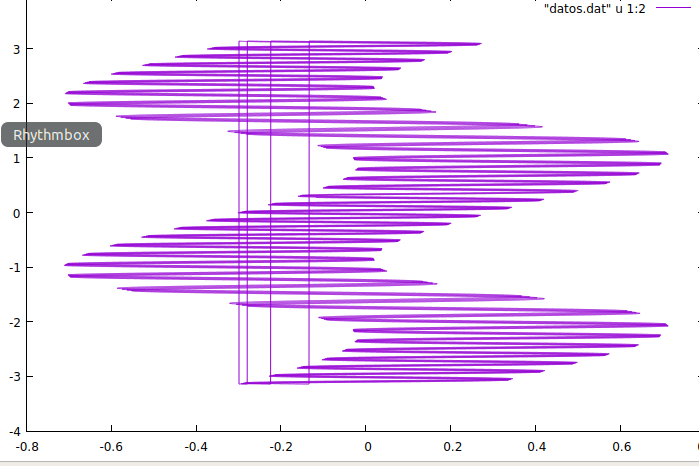
\includegraphics[scale=0.8]{1.PNG}
    \caption{$\theta_1$ vs $\theta_2$}
\end{figure}

\begin{figure}
    \centering
    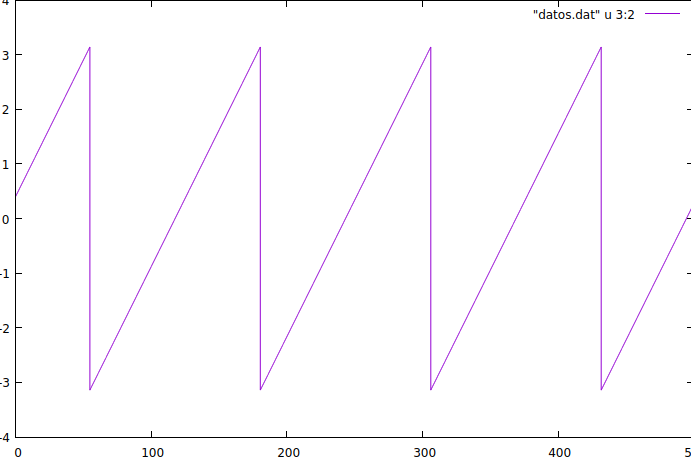
\includegraphics[scale=0.8]{2.PNG}
    \caption{$t$ vs $\theta_2$}
\end{figure}






\end{document}
